\documentclass[tikz]{standalone}

\usepackage{tkz-euclide}
\begin{document}
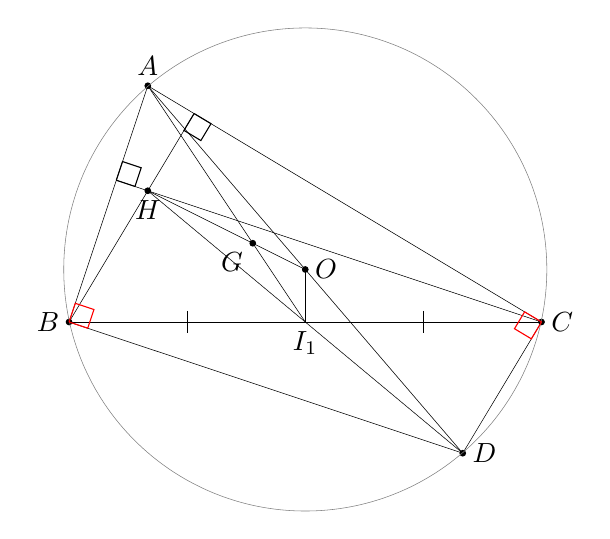
\begin{tikzpicture}
    \tkzDefPoints{0/3/A, -1/0/B, 5/0/C}
    
    % H point
    \tkzDefLine[perpendicular=through A, K=-1](B,C)
    \tkzGetPoint{h_1}
    \tkzInterLL(A,h_1)(B,C)
    \tkzGetPoint{H_1}
    \tkzDefLine[perpendicular=through B, K=-1](C,A)
    \tkzGetPoint{h_2}
    \tkzInterLL(B,h_2)(C,A)
    \tkzGetPoint{H_2}
    \tkzDefLine[perpendicular=through C, K=-1](A,B)
    \tkzGetPoint{h_3}
    \tkzInterLL(C,h_3)(A,B)
    \tkzGetPoint{H_3}
    \tkzInterLL(A,H_1)(B,H_2)
    \tkzGetPoint{H}

    % G point
    \tkzDefMidPoint(B,C)\tkzGetPoint{I_1}
    \tkzDefMidPoint(C,A)\tkzGetPoint{I_2}
    \tkzInterLL(A,I_1)(B,I_2)\tkzGetPoint{G}

    % O point
    \tkzDefLine[perpendicular=through I_1, K=-1](B,C)\tkzGetPoint{i_1}
    \tkzDefLine[perpendicular=through I_2, K=-1](C,A)\tkzGetPoint{i_2}
    \tkzInterLL(I_1,i_1)(I_2,i_2)\tkzGetPoint{O}

    \tkzDefCircle(A,B,C)
    
    \tkzInterLC(A,O)(O,A)\tkzGetPoints{A}{D}

    \tkzDrawSegments(A,B B,C C,A)
    \tkzDrawSegments(B,H_2 C,H_3 A,I_1 H,O O,I_1 A,D B,D C,D H,D)
    \tkzDrawPoints[fill=black](A, B, C, H, G, O, D)
    \tkzDrawCircle(O,A)

    \tkzMarkRightAngle(C,H_3,A)
    \tkzMarkRightAngle(B,H_2,C)
    \tkzMarkRightAngle[red](A,C,D)
    \tkzMarkRightAngle[red](A,B,D)
    \tkzMarkSegments(B,I_1 I_1,C)
    
    \tkzLabelPoint[above](A){$A$}
    \tkzLabelPoint[left](B){$B$}
    \tkzLabelPoint[right](C){$C$}
    \tkzLabelPoint[below](H){$H$}
    \tkzLabelPoint[below left](G){$G$}
    \tkzLabelPoint[right](O){$O$}
    \tkzLabelPoint[below](I_1){$I_1$}
    \tkzLabelPoint[right](D){$D$}
\end{tikzpicture}
\end{document}